\documentclass{article}
\usepackage[utf8]{inputenc}
\usepackage{geometry}
\usepackage{datetime2}
\usepackage{xparse}
\usepackage{amsmath}
\usepackage{booktabs}
\usepackage{array}
\usepackage{hyperref}
\usepackage{minted}

 \geometry{
 a4paper,
 total={170mm,257mm},
 left=20mm,
 top=20mm,
 }

 
 \usepackage{graphicx}
 \usepackage{titling}

 \title{Temporal plot of P3DX joint velocity and body velocity
}
% \author{Muhammad Qomaruz Zaman}
\date{18 March 2026}
 
 \usepackage{fancyhdr}
\fancypagestyle{plain}{%  the preset of fancyhdr 
    \fancyhf{} % clear all header and footer fields
    \fancyfoot[R]{}
    \fancyfoot[L]{}
    \fancyhead[L]{
\includegraphics[width=2cm]{ITS_pojok.pdf}}
    \fancyhead[R]{ \DTMnow}
}
\makeatletter
\def\@maketitle{%
  \newpage
  \null
  \vskip 1em%
  \begin{center}%
  \let \footnote \thanks
    {\LARGE \@title \par}%
    \vskip 1em%
    %{\large \@date}%
  \end{center}%
  \par
  \vskip 1em}
\makeatother

\usepackage{lipsum}  
% \usepackage{cmbright} % Change the font by zee

\begin{document}

\maketitle


\noindent\begin{tabular}{@{}ll}
    Author(s): & Muhammad Bari Akmal\\
     Teacher: &  Muhammad Qomaruz Zaman, S.T., M.T., Ph.D.\\
     Class name: & Sistem Robot Otonom\\
     YouTube video link: & \url{https://youtu.be/lkS01gzkMho} \\
     GitHub link: & \url{https://github.com/huggingface/datasets.git}
\end{tabular}
\vspace{2cm}


Pada tugas ini, digunakan model robot P3DX sebagai objek simulasi dan CoppeliaSim sebagai aplikasi untuk melakukan simulasi. Kode pyhton digunakan agar CoppeliaSim memberikan data perilaku model robot P3DX pada bagian terminal CoppeliaSim secara real time. Pergerakkan model robot P3DX dapat dilihat pada link youtube pada dokumen ini. Untuk mendapatakn data Joint Velocity, digunakan kode python sebagai berikut

\begin{minted}[frame=lines, framesep=2mm, linenos]{python}
import time
import math
import numpy as np
import matplotlib.pyplot as plt
from datetime import datetime
from coppeliasim_zmqremoteapi_client import RemoteAPIClient

client = RemoteAPIClient()
sim = client.require('sim')

sim.startSimulation()
print("Simulation Started")

p3dx_RW = sim.getObject("/PioneerP3DX/rightMotor")
p3dx_LW = sim.getObject("/PioneerP3DX/leftMotor")

rw = 0.195/2
rb = 0.381/2
d = 0.05

try:
    start_time = time.time()
    while (time.time() - start_time) < 10:
        
        elapsed = time.time() - start_time
        print(f"Running... {elapsed:.1f}s", end="\r")
        
        wr_vel = sim.getJointTargetVelocity(p3dx_RW)
        wl_vel = sim.getJointTargetVelocity(p3dx_LW)

        sim.addLog(1, f"RW:{wr_vel:.1f}, LW:{wl_vel:.1f}")

finally:
    sim.stopSimulation()
    print("\nSimulation Stopped")
\end{minted}

Setelah kode diatas di run, maka nilai joint velocity akan muncul pada terminal CoppeliaSim dan didapatkan
grafik joint velocity sebagai berikut:

\begin{figure}[H]
    \centering
    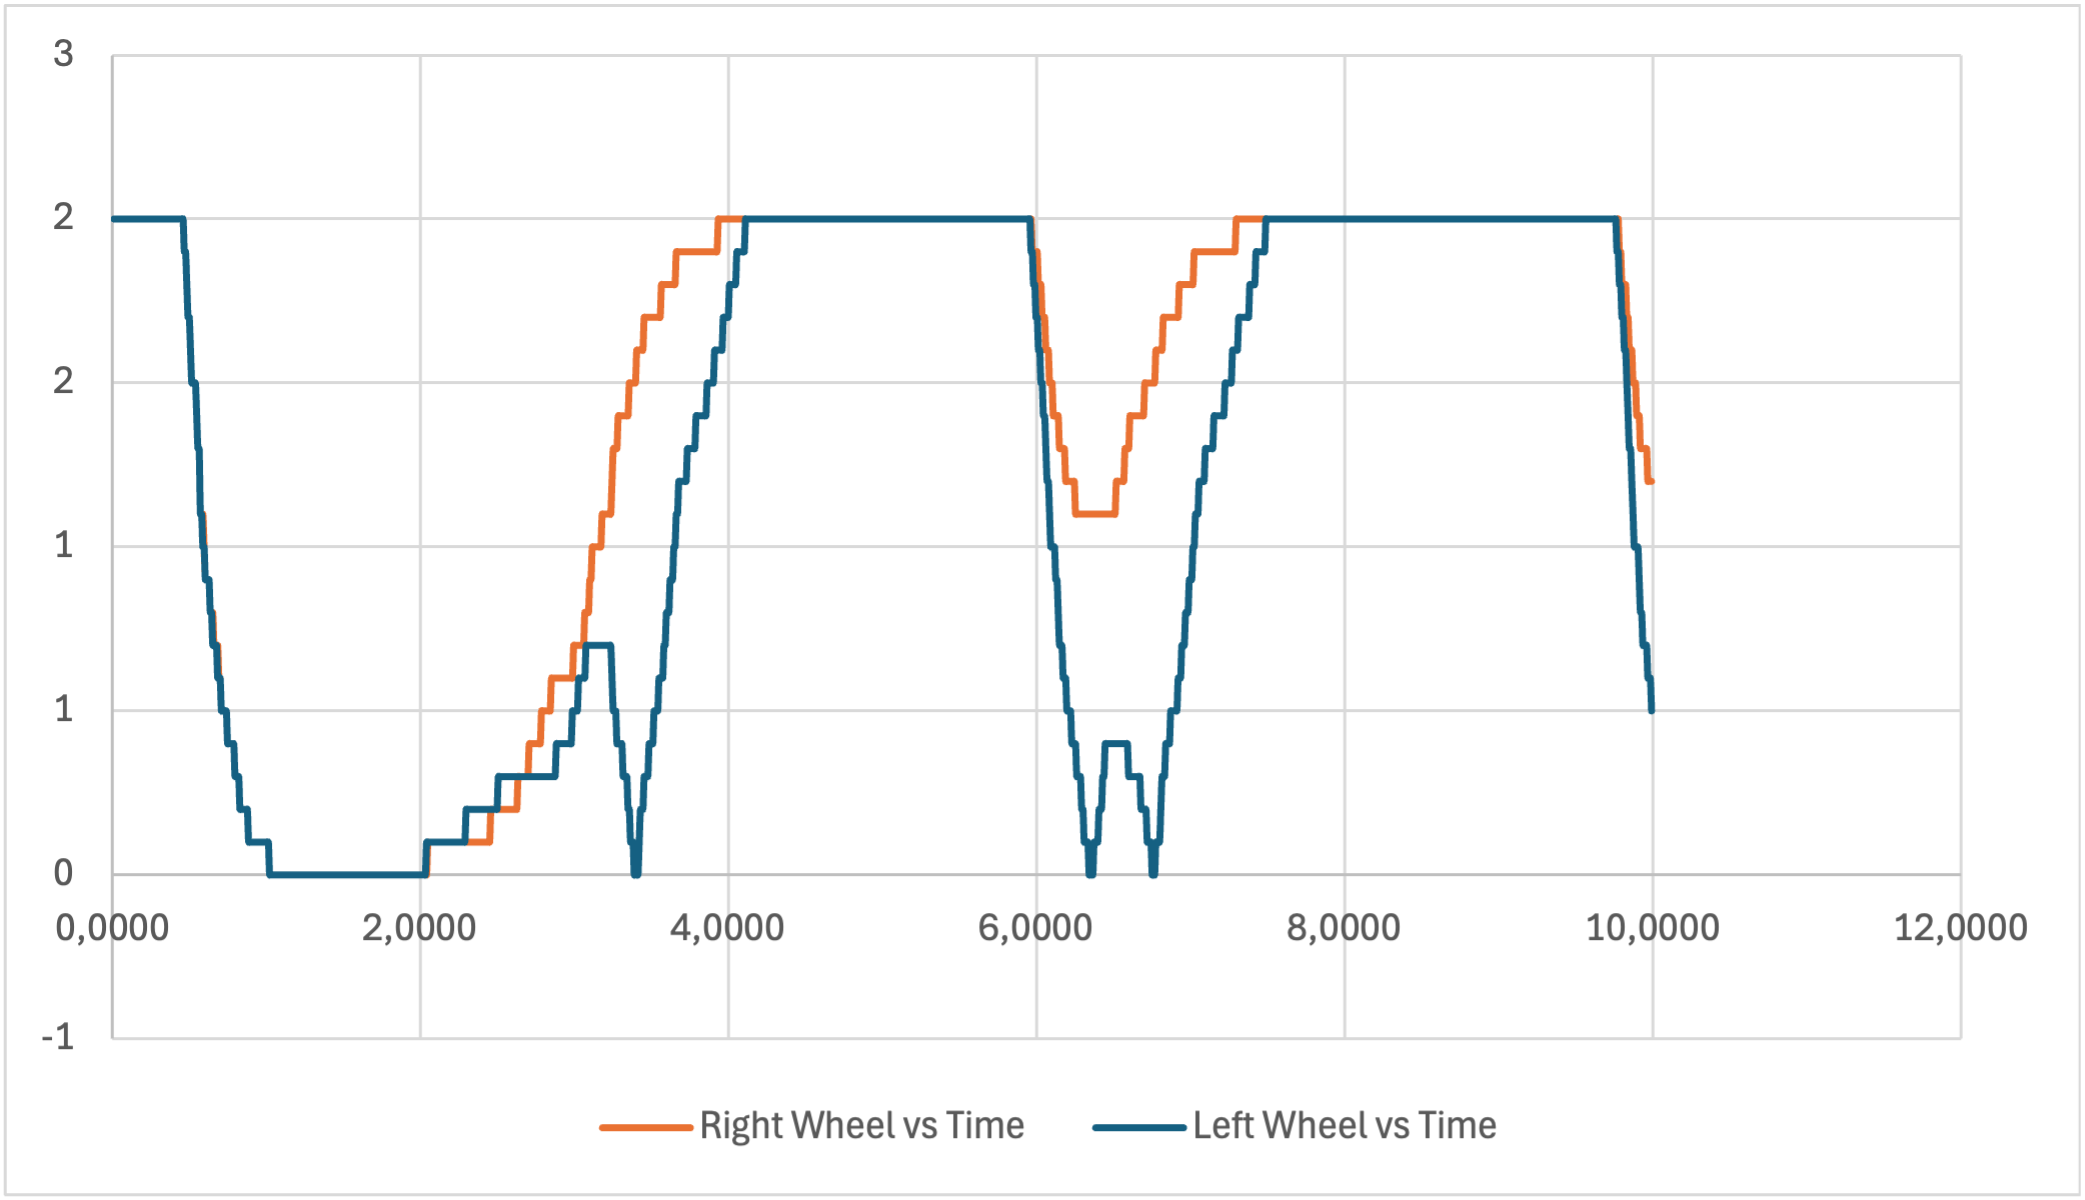
\includegraphics[width=0.5\linewidth]{Joint_vel.png}
    \caption{Grafik Joint Velocity Terhadap Waktu}
    \label{fig:enter-label}
\end{figure}

Lalu, digunakan kode python dibawah untuk mendapat nilai body velocity sebagai berikut

\begin{minted}[frame=lines, framesep=2mm, linenos]{python}
import time
import math
import numpy as np
import matplotlib.pyplot as plt
from datetime import datetime
from coppeliasim_zmqremoteapi_client import RemoteAPIClient

client = RemoteAPIClient()
sim = client.require('sim')

sim.startSimulation()
print("Simulation Started")

p3dx_RW = sim.getObject("/PioneerP3DX/rightMotor")
p3dx_LW = sim.getObject("/PioneerP3DX/leftMotor")

rw = 0.195/2
rb = 0.381/2
d = 0.05

try:
    start_time = time.time()
    while (time.time() - start_time) < 10:

        elapsed = time.time() - start_time
        print(f"Running... {elapsed:.1f}s", end="\r")
        
        wr_vel = sim.getJointTargetVelocity(p3dx_RW)
        wl_vel = sim.getJointTargetVelocity(p3dx_LW)

        vx = (wr_vel + wl_vel)*rw/rb
        wx = (wr_vel - wl_vel)*rw/rb

        sim.addLog(1, f"Vx:{vx:.1f}m/s, Wx:{wx:.1f}rad/s")

finally:
    sim.stopSimulation()
    print("\nSimulation Stopped")
\end{minted}

Setelah kode diatas di run, maka nilai joint velocity akan muncul pada terminal CoppeliaSim dan didapatkan
grafik body velocity sebagai berikut:

\begin{figure}[H]
    \centering
    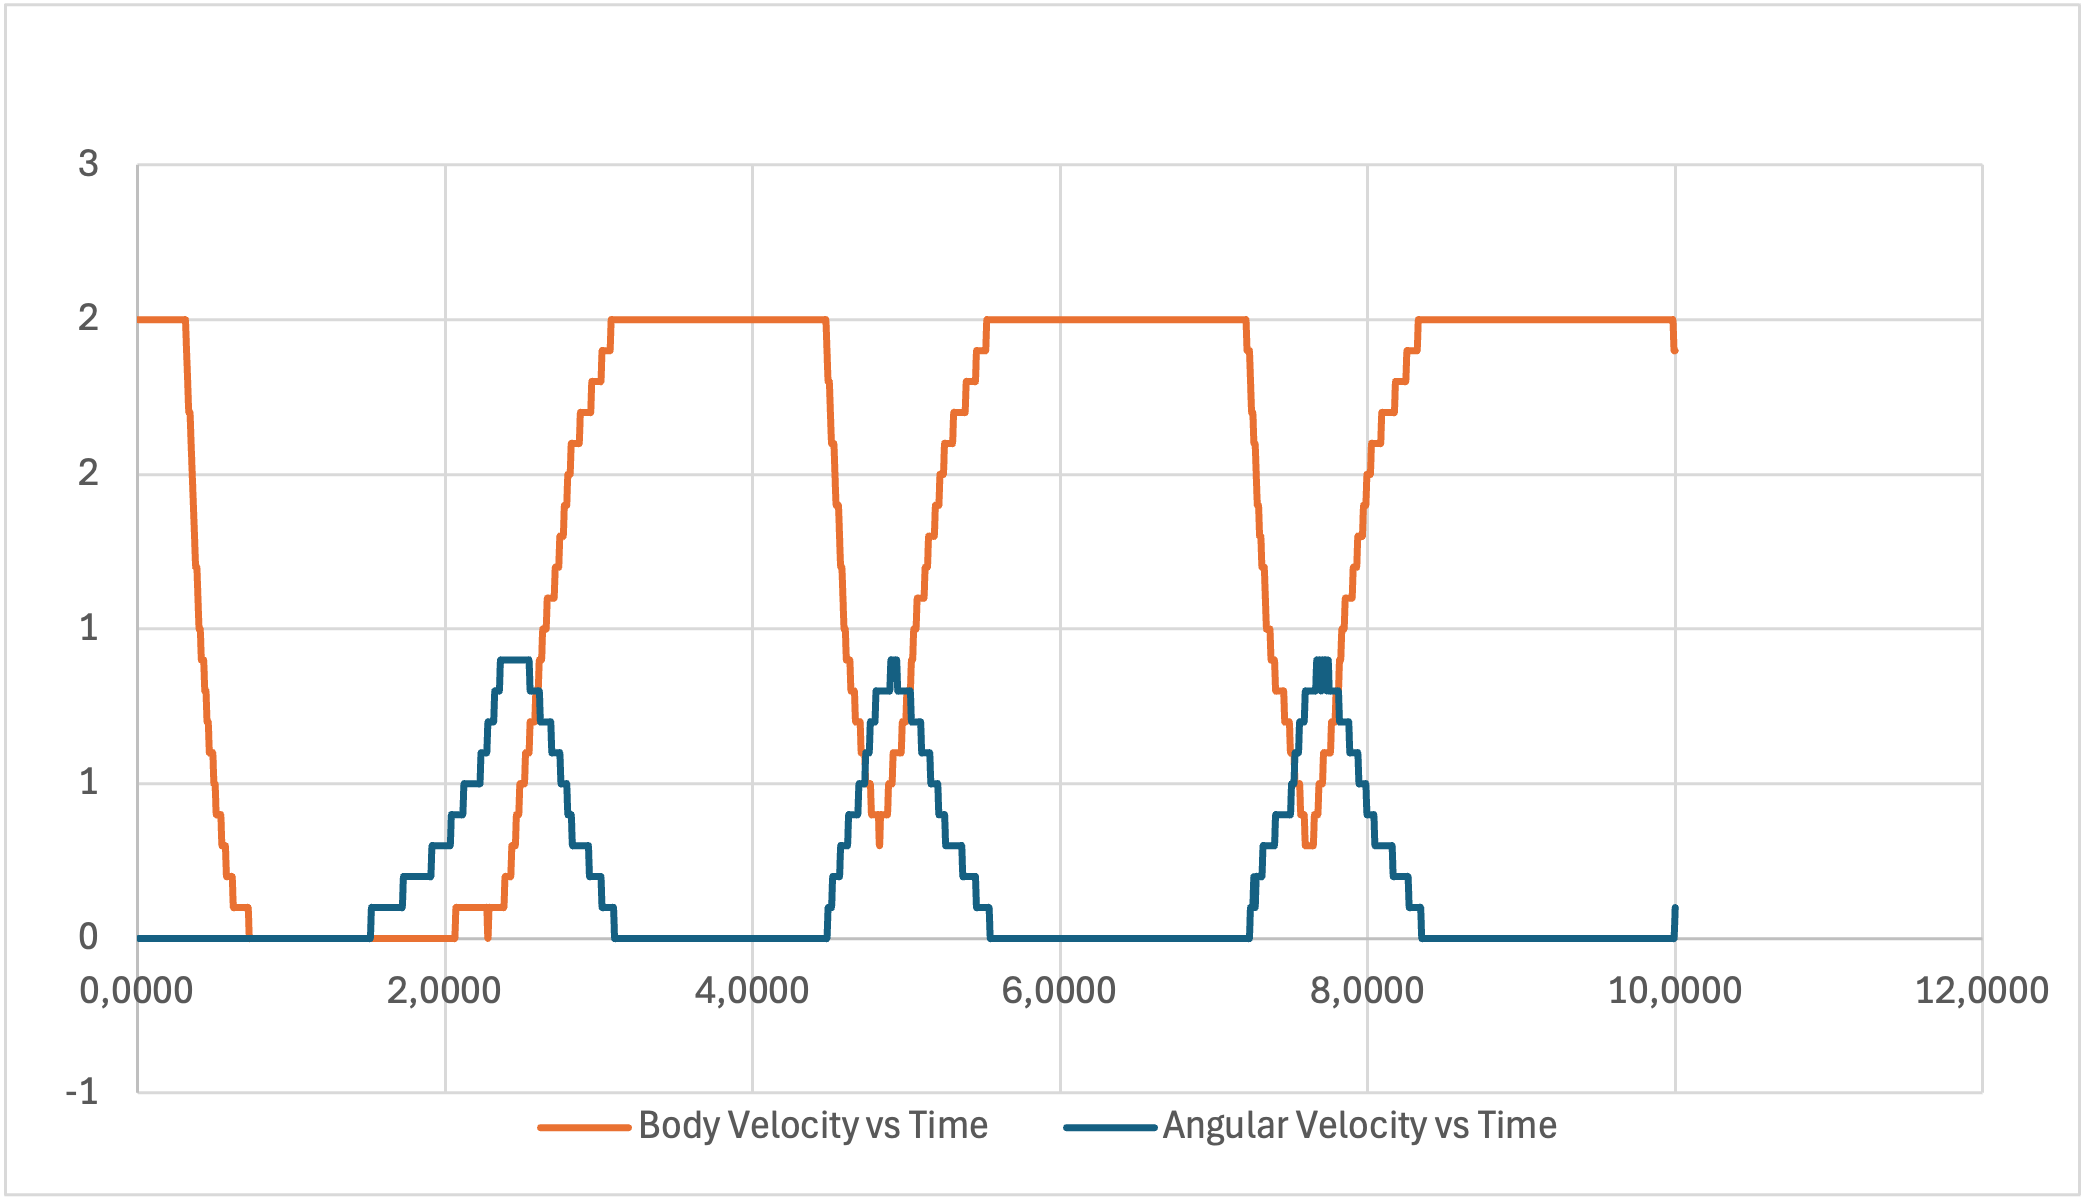
\includegraphics[width=0.5\linewidth]{Body_vel.png}
    \caption{Grafik Body Velocity Terhadap Waktu}
    \label{fig:enter-label}
\end{figure}

\end{document}
